\section{Evaluation}
This section of the report aims to  discuss and describe the information that
can be gained from the results goatherd in the previous section.
Evaluation of results is a critical step in determination of success of a
study, and ultimately answering the research question originally posed in
Section \ref{sec_res_q}.

\subsection{Robot}
Due to shortcomings of the Thymio II platform described in Section
\ref{meth_slam}, it was not possible to implement the required subtasks or
models needed to produce a valid SLAM solution.
As a result of this lack of implementation, it is not possible to provide a
formal evaluation of the system.

While the evaluation  of the SLAM implementation is not possible, it is still
possible to discuss the metrics that may have been utilised to quantify the
SLAM implementation.

As per previous studies conducted in the field of autonomous navigation, one of
the most common metrics of evaluation is a simple comparison of the robot's
estimated location of map features and itself, and the physical location of
said features.
It is crucial to remember that SLAM solutions are approximation techniques,
and as such a certain degree of error is expected within an robot's
estimations.

A second common metric or evaluation SLAM solutions is to measure the time
take for a robotic agent to map a certain percentage of an environment, or to
find a number of specific landmarks within said environment.
Timed metrics are often an unreliable evaluation technique, as robotic agents
can produce artificially high results with low accuracy SLAM solutions, by
simply moving at a faster speed through an environment.

Much like a SLAM solution itself, the techniques utilised in the evaluation of
an implementation must be tailored to system, the sensors utilised, the manner
of estimation, the type of map produced, and the specification of the robot.

One of the two sub-queries posed as a research question for this study was:
\begin{quote}
``Is it possible to implement a SLAM solution using a robot with limited or
primitive hardware?''
\end{quote}
While this study's inability is indicative of a negative answer to this
question, much of the literature reviewed in Section \ref{sec_slam} reveals
that implementation of SLAM solutions on primitive robotic platforms is in
fact possible.

In hindsight the original sub-query can be consider vague or leading, a more
suitable research question would have been:

\begin{quote}
``What are the hardware limitations to implementing a SLAM solution on a
mobile robotic platform?''
\end{quote}

While this revised research query cannot be answered by the results gained by
this study, it is certainly a more appropriate question, and a suitable topic
for a future investigation.


\subsection{Simulator}
\subsubsection{Memory Consumption}
\begin{figure}[!h]
    \centering
    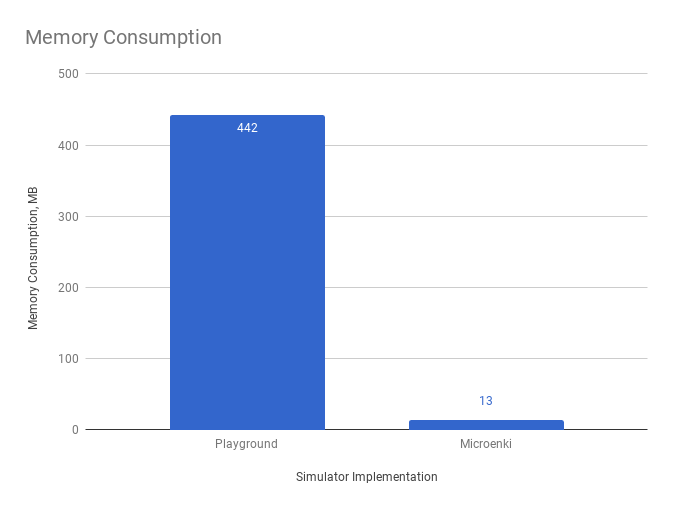
\includegraphics[width=\textwidth]{memory.png}
    \caption{Memory consumption for the simulator implementations}
\end{figure}
Following the benchmarking of the two implementations, we can compare their
memory consumption as shown. At 442 MB, the initial Playground simulator was a
fairly hefty application even on desktop environments, and is fairly unsuitable
for embedding onto any robotic platform to run autonomously.

The new simulator is much cut down, consuming only 13 MB in the steady state.
By constructing a simulator without any components not required for simulation
of tasks alone, such as the GUI, the executable image that the hardware
platform must host is much smaller. Additionally, runtime data such as models,
background textures are not required to be loaded from disk.

Overall, the new simulator is approximately 2.9\% of the size of Aseba
Playground, meaning that in practice, 34$\times$ as many instances may be
hosted in memory at any given time. If the simulations are memory constrained,
this presents a considerable increase in potential parallelism.

\subsubsection{CPU Consumption}
\begin{figure}[!h]
    \centering
    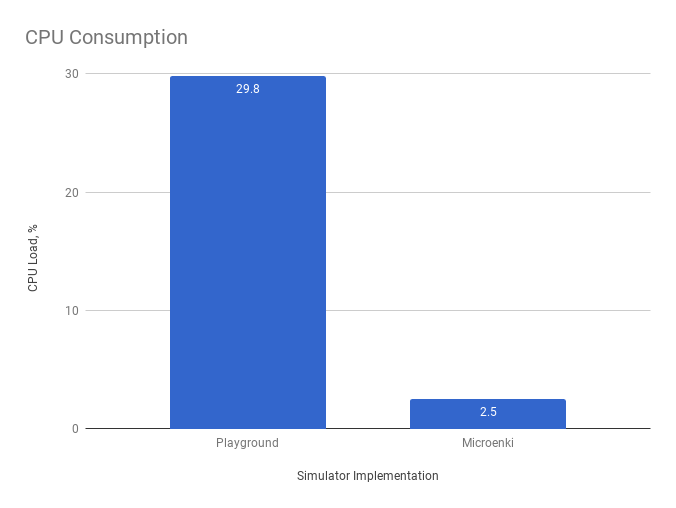
\includegraphics[width=\textwidth]{cpu.png}
    \caption{CPU consumption for the simulator implementations}
\end{figure}
While memory consumption determines how many simulations can be loaded at once,
the CPU consumption determines how many may be executed in simultaneously.

At the steady state, the Playground consumed 29.8\% of a single CPU core. In
comparison, the new simulator consumed at the steady state only 2.5\% of a CPU
core. These measurements render the new simulator at 8.4\% of the load, meaning
that you could execute 11$\times$ as many instances in parallel.

The difference in CPU load is not nearly as striking as the comparison between
the two simulators with regard to their memory consumption. This is because of
the relative split in requirements of various removed components. For example,
while the GUI has a very heavy memory cost, the amount of effort to execute the
code behind it is quite low. By removing the GUI components, we can quickly cut
memory without as much of an impact on the CPU.

\subsubsection{Simulation Ratio}
\begin{figure}[!h]
    \centering
    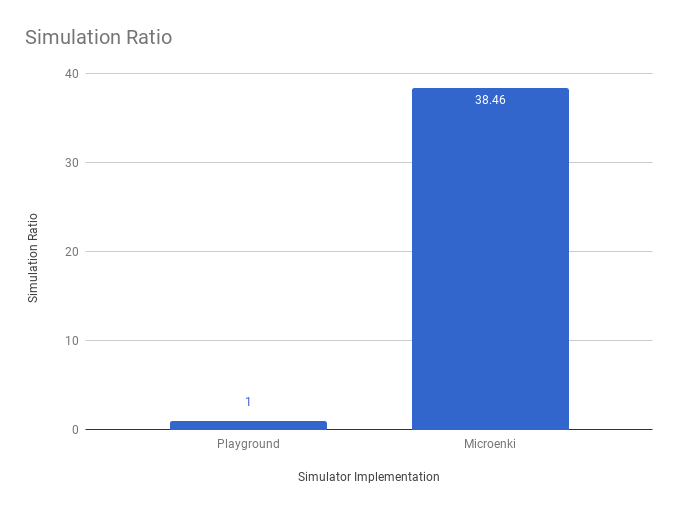
\includegraphics[width=\textwidth]{ratio.png}
    \caption{Simulation ratio for the simulator implementations}
\end{figure}
Where the CPU and memory consumption aspects of the results describe
improvements in potential parallelisation, the difference in simulation speed
ratio is directly linked to serial execution, or at least, the amount of time
taken to execute a simulation with fixed end conditions, such as total time, or
the completion of certain goals.

The Aseba Playground is designed primarily as an interactive application, where
a user can observe and interact with the simulation. Because of this, the
simulation is fixed at a 1:1 ratio, where the simulator tries to execute 1
second of simulation time per real life second. This allows the user intuitive
understanding of the lengths of time involved and eases interaction - greatly
increased speeds would make it impossible to manipulate the simulation
effectively.

As all interaction with the simulation in our target use cases will be
programmatic, we needn't make such considerations. Instead, we can remove any
kind of speed governing and execute as fast as possible. In testing, we were
able to observe a ratio of 38.46, meaning that for every real-world second,
the simulator was able to execute 38.46 seconds of simulator time. As the
Playground intends to always run at a fixed rate, it will not scale up or down
with processor speed, making direct comparison less important. More important
is that by removing both the speed governing functionality, and by reducing the
computational load of other components (such as graphical rendering), the new
simulator will run strictly at least as fast as the Playground, presenting a
pragmatic advantage in automated scenarios.
